% -*- TeX -*- -*- UK -*-
% ----------------------------------------------------------------
\documentclass[12pt]{article}
%Preamble:
\usepackage{a4wide}
\input{sl_preamble.tex}
\hypersetup{colorlinks,linkcolor=blue,citecolor=teal,urlcolor=teal}
\input{sl_graphics_preamble.tex}
\graphicspath{{"Figures/"}}
%
\usepackage{array}
\newcounter{tablerow}
\newcommand{\tablerowautorefname}{row}
\newenvironment{tabularn}[1]{\setcounter{tablerow}{0}\begin{tabular}{#1>{\refstepcounter{tablerow}}l}}{\end{tabular}}
%\usepackage{etoolbox}
%\AtBeginEnvironment{tabular}{\setcounter{tablerow}{0}}
%
% ----------------------------------------------------------------
% New commands etc.
\input{sl_definitions.tex}
\input{sl_symbols.tex}
%matrices
\newcommand{\I}{\mathbf{I}}
%vec of ones
%equilibrium distribution
\newcommand{\pr}{\mathbf{p}}
\newcommand{\eq}{\pr^\infty}
%other symbols
\newcommand{\w}{\mathbf{w}}
\newcommand{\W}{\mathbf{W}}
\newcommand{\frg}{\W^\mathrm{F}}
\newcommand{\M}{\mathbf{M}}
\newcommand{\F}{\boldsymbol{\Phi}}
\newcommand{\pot}{^{\text{pot}}}
\newcommand{\dep}{^{\text{dep}}}
\newcommand{\potdep}{^{\text{pot/dep}}}
\newcommand{\norm}{_0}
\newcommand{\inc}{_{\text{inc}}}
\newcommand{\dec}{_{\text{dec}}}
\newcommand{\incdec}{_{\text{inc/dec}}}
\newcommand{\wt}{_{\text{WT}}}
%\newcommand{\ko}{_{\text{D$^\mathrm{b}$K$^\mathrm{b}$-/-}}}
\newcommand{\KO}{D$^\mathrm{b}$K$^{\mathrm{b}-/-}$}
\newcommand{\ko}{_{\text{MHC}}}
%\newcommand{\KO}{MHC}
\newcommand{\tpre}{t_{\text{pre}}}
\newcommand{\ttrain}{t_{\text{train}}}
\newcommand{\lmax}{_{\text{max}}}
\newcommand{\lmin}{_{\text{min}}}
% ----------------------------------------------------------------
%
%%%%%%%%%%%%%%%%%%%%%%%%%%%%%%%%%%%%%%%%%%%%%%%%%%%%%%%%%%%%%%%%%%%%%%%%%%
% Title info:
\title{A saturation model for impaired learning with enhanced plasticity: Supplementary material}
%
%% Author List:
%%
%\author{An Author$^a$, Another Author$^b$ and Yet Another Author$^c$\\
%%
%\small{\emph{$^a$ Address 1}}\\
%\small{\emph{$^b$ Address 2}}\\
%\small{\emph{$^c$ Address 3}}\\
%}
\date{}

\begin{document}

\maketitle


%%%%%%%%%%%%%%%%%%%%%%%%%%%%%%%%%%%%%%%%%%%%%%%%%%%%%%%%%%%%%%%%%%%%%%%%%%


%\begin{abstract}
%  We see if we can model VOR gain increase and decrease learning in mice with a knockout in MHC as well as wild-type.
%\end{abstract}

\tableofcontents
\listoffigures

%%%%%%%%%%%%%%%%%%%%%%%%%%%%%%%%%%%%%%%%%%%%%%%%%%%%%%%%%%%%%%%%%%%%%%%%%%
% Beginning of Article:
%%%%%%%%%%%%%%%%%%%%%%%%%%%%%%%%%%%%%%%%%%%%%%%%%%%%%%%%%%%%%%%%%%%%%%%%%%

\section{Mathematical formalism}\label{sec:setup}


\subsection{Models of synapses}\label{sec:synapse}

We make the following assumptions:
\begin{itemize}
  \item There are $N$ identical synapses with $M$ internal functional states.
  \item The states of different synapses are independent of each other.
  \item The synapses that are eligible for plasticity are chosen randomly.
  \item Candidate potentiating/depressing plasticity event timings are distributed as Poisson processes with rates $r\potdep$.
  \item Potentiation and depression are described by Markov processes with transition probabilities $\M\potdep$.
  \item The synaptic weights of the internal states are given by the column vector $\w$. This can only take values in a finite range that we can shift to $\pm1$. Most of the models will only use the two extreme values.
\end{itemize}

In practice, the overall rate of candidate plasticity events will only set the timescale, and only the relative rates will matter.
With this in mind, we define
%
\begin{equation}\label{eq:fpotdep}
  r = r\pot + r\dep,
  \qquad
  f\pot = \frac{r\pot}{r},
  \qquad
  f\dep = \frac{r\dep}{r}.
\end{equation}
%
The quantities $f\potdep$ measure the fraction of candidate plasticity events that are potentiating/depressing.

The independence and identicalness of synapses means that the state of the system can be completely described by the probability distribution of the internal states, the row vector $\pr(t)$.

The evolution of this probability is described by a continuous time Markov matrix matrix, $\frg$:
%
\begin{equation}\label{eq:evolve}
  \diff{\pr(t)}{t} = r\pr(t)\frg,
  \qquad
  \frg = f\pot\M\pot+f\dep\M\dep-\I,
\end{equation}
%
where $\I$ is the identity matrix.
Eventually, this will settle into the equilibrium distribution:
%
\begin{equation}\label{eq:eqprob}
  \eq\frg=0.
\end{equation}
%

For models with only two possible synaptic weights, the distribution of synaptic weights is completely described by the mean, $\pr(t)\w$.


The \KO\ mice have a lower threshold for depression.
We can model this by changing $\M\dep\wt$ to $\M\dep\ko$, which should have larger off-diagonal matrix elements.

We will look at several different models,
the serial model (see \cite{Leibold2008serial} and \autoref{fig:models}\ref{fig:serial_model}) which has only two values for the synaptic weight,
the two-state model (which can be thought of as a special case of the serial model, see \autoref{fig:models}\ref{fig:binary_model}),
the multistate model (see \cite{amit1994learning,Fusi2007multistate} and \autoref{fig:models}\ref{fig:multistate_model}) which has a linearly varying synaptic weight,
and the cascade model (see \cite{Fusi2005cascade} and \autoref{fig:models}\ref{fig:cascade_model}).
We will also look at a new, pooled resource model that we will define below in \autoref{sec:pooledmodel} and a non-uniform version of the multistate model that we will describe in \autoref{sec:nonunimodel}.

For the serial, multistate and two state models, we will use the same value for the transition probabilities, $q$, for potentiation and depression in the wild-type as well as potentiation in the \KO\ models.
We will use a larger value for $q$ for depression in the \KO\ models.

For the cascade model, we will use the same value for the parameter $x$ (which controls the decay of transition rates, see \cite{Fusi2005cascade}) for potentiation and depression in the wild-type as well as potentiation in the \KO\ models.
We will use a larger value for $x$ for depression in the \KO\ models.

The values used for all these parameters in simulations are listed in \autoref{tab:params}.

\begin{figure}
 \begin{center}
 \parbox{0.8\linewidth}{%
 \begin{myenuma}
  \item\aligntop{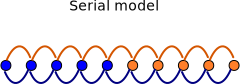
\includegraphics[height=1.7cm]{serial.svg}}\label{fig:serial_model}\hspace{0.5cm}
  \item\aligntop{\includegraphics[height=1.7cm]{binary.svg}}\label{fig:binary_model}\hspace{0.5cm}\\[1cm]
  \item\aligntop{\includegraphics[height=1.7cm]{multistate.svg}}\label{fig:multistate_model}\hspace{0.5cm}
  \item\aligntop{\includegraphics[height=2.5cm]{cascade.svg}}\label{fig:cascade_model}
 \end{myenuma}
 }
 \end{center}
  \caption[Transition probabilities for different models]{Transition probabilities for different models.
  Potentiation induces transitions indicated by orange arrows, depression indicated by blue arrows.
  States of strong/weak synaptic weight indicated by orange/blue circles.
  (\ref{fig:serial_model}) In the serial model the transition probabilities for potentiation/depression are all equal and it is parameterised by these two values.
  The synaptic weight takes only two values, $\pm1$.
  (\ref{fig:binary_model}) The two-state model is parameterised by the two transition probabilities.
  (\ref{fig:multistate_model}) In the multistate model the transition probabilities for potentiation/depression are all equal and it is parameterised X
  by these two values.
  The synaptic weight varies linearly in the interval $[-1,1]$.
  (\ref{fig:cascade_model}) In the cascade model, the transition probabilities decay geometrically with a parameter $x$ (see \cite{Fusi2005cascade}) and synaptic weight takes only two values.
  } \label{fig:models}
\end{figure}

\subsubsection{Pooled resource model}\label{sec:pooledmodel}

Suppose that there is some resource required for potentiation/depression that is shared between $P$ synapses and is depleted as more synapses are potentiated/depressed and replenished when this is reversed.
We can avoid going beyond the independent synapse model by modelling this pool of synapse as a single compound synapse.

We will model the individual synapses with the two-state model.
Let $i=0\ldots P$ be the number of them that are potentiated.
We will model the effect of resource depletion linearly with the potentiation/depression probabilities for the individual synapses:
%
\begin{equation}\label{eq:depletion}
  \begin{aligned}
    q\pot &= \frac{(P-i-1)q\lmax + i\,q\lmin}{P-1}, \quad& i &= 0 \ldots P-1,\\
    q\dep &= \frac{(i-1)q\lmax + (P-i)q\lmin}{P-1}, & i &= 1 \ldots P.
  \end{aligned}
\end{equation}
%
At each plasticity event for the compound synapse, one of the individual synapses will be chosen randomly for update.
This effectively reduces the transition probabilities by $1/P$.

This compound synapse would seem to have $2^P$ internal states.
However, we need only keep track of the number of potentiated synapses, not their identity, leaving $M=P+1$ states.
The transition network will then have a multistate topology (see \autoref{fig:models}\ref{fig:multistate_model}) but the transition probabilities will no longer be uniform and the weight of the compound synapse is the mean of its constituent synapses:
%
\begin{equation}\label{eq:pooledweight}
  \w_i = \frac{2i}{P}-1.
\end{equation}
%


The Markov process is lumpable \wrt this partition of states (see \cite[\S6.3]{kemeny1960finite} for the discrete time version and \cite{burke1958markovian,Ball1993Lumpability} for continuous time).
The transition probabilities between lumps $i$ and $j$ is computed by choosing one state from lump $i$ and summing the transition probabilities to all states in lump $j$.
The result must be the same for all states in lump $i$.

For any state in lump $i$, there are $P-i$ synapses that can be potentiated to go to lump $i+1$.
Each of these transition probabilities is $q\pot/P$.
Similarly, there are $i$ synapses that can be depressed to go to lump $i-1$.
Each of these transition probabilities is $q\dep/P$.
Thus:
%
\begin{equation}\label{eq:pooledpotdep}
  \begin{aligned}
    \M\pot_{ii+1} &=  \brk{\frac{(P-i-1)q\lmax + i\,q\lmin}{P-1}} \frac{P-i}{P} ,
      \quad& i &= 0 \ldots P-1,\\
    \M\dep_{ii-1} &=  \brk{\frac{(i-1)q\lmax + (P-i)q\lmin}{P-1}} \frac{i}{P} ,
           & i &= 1 \ldots P,
  \end{aligned}
\end{equation}
%
with all other off-diagonal elements equal to zero.
The diagonal elements are chosen so that the rows sum to one.

This model is parameterised by the range of values, $q\in[q\lmin,q\lmax]$, for potentiation and depression.
We will use the same values for potentiation and depression in the wild-type as well as potentiation in the \KO\ models.
We will use larger values for depression in the \KO\ models.
In the main text, we consider a version of this model that has resource depletion for depression only, so that potentiation transition probabilities are unaffected by the number of potentiated synapses.
This is done by setting $q\pot\lmax=q\pot\lmin$.
The values of these parameters are listed in \autoref{tab:params}.


\begin{figure}
 \begin{center}
  \aligntop{\includegraphics[height=4cm]{pooled.svg}}
 \end{center}
  \caption[The pooled resource model]{The pooled resource model.
  Several two-state synapses share resources that are required for potentiation and depression.
  These resources are depleted as more synapses are potentiated or depressed.
  This pool of synapses can be modelled as one compound synapse.} \label{fig:pooled_model}
\end{figure}


\subsubsection{Non-uniform multistate model}\label{sec:nonunimodel}

This model is similar to the multistate model (see \autoref{fig:models}\ref{fig:multistate_model})), as it only has transitions between adjacent states and a linearly varying synaptic weight.
However, like the cascade model (see \cite{Fusi2005cascade} and \autoref{fig:models}\ref{fig:cascade_model}), the transition probabilities decay exponentially away from the central transition.
More precisely:
%
\begin{equation}\label{eq:nonunidef}
    \M\pot_{ii+1} = \M\dep_{i+1i} =  x^{\abs{\frac{M+1}{2}-i}+\half},
      \quad i = 1 \ldots M-1,
\end{equation}
%
with all other off-diagonal elements equal to zero.
The diagonal elements are chosen so that the rows sum to one.

This model is parameterised by the values of $x$ chosen for potentiation and depression.
We will use a larger value for depression in the \KO\ models.
The values used are listed in \autoref{tab:params}.



\begin{figure}
 \begin{center}
  \aligntop{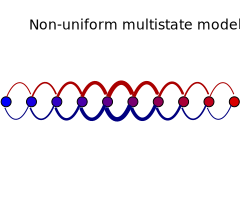
\includegraphics[height=3cm]{multistate_nonuni.svg}}
 \end{center}
  \caption[The non-uniform multistate model]{The non-uniform multistate model.
  Similar to the multistate model, \autoref{fig:models}\ref{fig:multistate_model}), the synaptic weight varies linearly in the interval $[-1,1]$, but the transition probabilities between adjacent states decays exponentially away from the central transition for both potentiation and depression.} \label{fig:nonuni_model}
\end{figure}



\subsection{Model of VOR learning experiment}\label{sec:learning}

Training the animal will not change the internal dynamics of a synapse under potentiation or depression.
It will change the environment, which will lead to a change in how often potentiation and depression occur.
It could be manifested in a change in which synapses are potentiated/depressed, but this could not be captured in this type of model.
We will model this by changing $f\potdep$, leaving $\M\potdep$ unchanged.
This approach was used to model motor learning in \cite{Smith2006savings}.

The untrained case will be described by $f\dep=f\dep\norm$.
Gain-increase training  will be described by $f\dep=f\dep\inc>f\dep\norm$, and
gain-decrease training  will be described by $f\dep=f\dep\dec<f\dep\norm$.
Note that the forgetting matrix \eqref{eq:evolve} and the equilibrium distribution \eqref{eq:eqprob} depend on $f\dep$, which we will indicate with subscripts.

Before training, the synaptic distribution will be in the equilibrium distribution corresponding to $f\dep\norm$.
During gain-increase training, it will evolve according to \eqref{eq:evolve} with $f\pot\inc$:
%
\begin{equation}\label{eq:nopre}
  \pr(t) = \eq\norm \exp\prn{rt\frg\inc}.
\end{equation}
%
On the other hand, if the gain-increase training follows gain-decrease pre-training for some time period, $\tpre$:
%
\begin{equation}\label{eq:withpre}
  \pr(t) = \eq\norm \exp\prn{r\tpre\frg\dec} \exp\prn{r(t-\tpre)\frg\inc}.
\end{equation}
%

We will describe the effect of training by the decrease in mean synaptic weight:
%
\begin{equation}\label{eq:learning}
  L(t) = \prn{\pr(0)-\pr(t)}\w.
\end{equation}
%
If we imagine something like an LN model for the Purkinje cell, the output would depend on some linear combination of the synaptic weights (weighted by the activities of the corresponding parallel fibres).
If we're not keeping track of synaptic identity, the most natural linear combination to use would be an equal sum of them all.
The behavioural output (VOR gain) will be some unknown, non-linear function of the synaptic weights, so the best we can hope for is to reproduce qualitative features of the experiment, such as whether learning is enhanced or impaired by the mutation or pre-training.

We will assume $f\dep\wt=f\dep\ko$.
This is because the effects of the mutation are well localised to the Purkinje cells, so the activity of the parallel and climbing fibres should not change very much.
Therefore the rates of potentiation and depression should not change very much either.
This implies that the mean synaptic weight in equilibrium differs between the \KO\ models and wild type, but that is also suggested by the data regarding basal levels of phospho-GluR2 at serine 880.
As the mutation produces no change in baseline performance, there must be a compensatory mechanism somewhere else.
We will model this compensation as a simple linear offset, as could be produced by another population of neurons/synapses whose effect cancels with these neurons/synapses.

For the most part, we set $f\dep\norm=\half$, $f\dep\inc=f\dep\norm+\Delta f$ and $f\dep\dec=f\dep\norm-\Delta f$, with $\Delta f>0$.
We use the same values for wild-type and \KO\ models for the reasons discussed above.
We will mostly treat gain-increase and decrease symmetrically, but this is not necessary.
We could adjust $r$ to keep $r\pot$ unchanged, if so desired, but this would only change the overall timescale and would not affect any of the qualitative comparisons that we are concerned with here.
The values of these parameters are listed in \autoref{tab:params}.

We are also assuming that the relation between VOR gain and mean synaptic weight is the same for \KO\ mice and wild-type, except for a linear offset to compensate for the difference in equilibrium weights mentioned above.
This ensures that the qualitative questions mentioned above (enhancement or impairment of learning) will not be affected.




\section{Simulation and analysis of models}\label{sec:results}

The features of the actual experiments that we'd like to capture are:
\begin{enumerate}
  \item Without pre-training, gain-increase learning is significantly faster in the wild-type than in the \KO\ mice.
  \item For the wild-type, gain-increase learning is significantly faster without pre-training than with it.
  \item For the \KO\ mice, gain-increase learning is significantly faster with pre-training than without it.
  \item After pre-training, gain-increase learning is significantly faster in the \KO\ mice than in the wild-type.
  \item Gain-decrease pre-training is slightly faster in the wild-type, but not significantly so.\label{it:gaindown}
\end{enumerate}
These questions will not be affected by any output nonlinearity, as long as it is monotonic and fixed.
We will not worry too much about \autoref{it:gaindown}, as gain-decrease learning uses a different mechanism to gain-increase.
We are only modelling the effect of gain-decrease training on \emph{these} synapses.

We will not worry too much about the curvature of the learning curves, as this can be changed by the nonlinear relation between synaptic weight and VOR gain.
However, both the wild-type and \KO\ mice should be affected in the same way, so the difference in the curvature of the \KO\ mice and wild-type curves after pre-training would be nice to capture.

We will try to gain some analytic insight to some of these models by looking at the slope of the learning curve at the start of gain-increase training.
This is proportional to the net-flux from the states with strong synaptic weight to the weaker states, measured using the transition probabilities for gain-increase but the equilibrium distribution for either untrained or gain-decrease, assuming that pre-training lasts long enough to reach the equilibrium distribution for gain-decrease.
This should be multiplied by the difference in synaptic weights.
But, as this quantity is constant within a model and doesn't change when comparing wild-type and \KO\ models or with/without pre-training, it can be ignored.

The values for all parameters we will use can be found in \autoref{tab:params}.


\begin{table}
 \begin{center}
  \begin{tabularn}{|l|c|c|c|c|c|c|}
    \cline{1-7}
    % after \\: \hline or \cline{col1-col2} \cline{col3-col4} ...
    Model & \# states & pot & WT dep & \KO\ dep & $\Delta f$ & $r\tpre$ \\
    \cline{1-7}
    Serial        & 10 & $q=0.3$  & $q=0.3$  & $q=0.4$  & 0.1  & 20  &\label{tr:multistate_weak} \\
    Serial        & 10 & $q=0.3$  & $q=0.3$  & $q=0.4$  & 0.3  & 20  &\label{tr:multistate_med} \\
    Serial        & 10 & $q=0.3$  & $q=0.3$  & $q=0.4$  & 0.45 & 30  &\label{tr:multistate_strong} \\
    Two-state     & 2  & $q=0.1$  & $q=0.1$  & $q=0.2$  & 0.1  & 5   &\label{tr:binary} \\
    Multistate    & 10 & $q=0.3$  & $q=0.3$  & $q=0.4$  & 0.3  & 5   &\label{tr:multistate_lin} \\
%    Pooled        & 10 & $q\in[0.3,0.4]$  & $q\in[0.3,0.4]$  & $q\in[0.6,0.8]$
%                                          & 0.1 & 20 &\label{tr:pooled_plenty}\\
%    Pooled        & 10 & $q\in[0.05,0.4]$ & $q\in[0.05,0.4]$  & $q\in[0.1,0.8]$
%                                          & 0.1 & 20 &\label{tr:pooled_scarce}\\
    Pooled res. & 7  & $q=0.008$        & $q\in[0.0006,0.6]$  & $q\in[0.001,1]$
                                          & 0.4 & 20 &\label{tr:pooled_deponly}\\
    Cascade       & 10 & $x=0.25$ & $x=0.25$ & $x=0.33$ & 0.3  & 20  &\label{tr:cascade_short} \\
    Cascade       & 10 & $x=0.25$ & $x=0.25$ & $x=0.33$ & 0.3  & 100 &\label{tr:cascade_long} \\
    Non-uni. MS& 10 & $x=0.25$ & $x=0.25$ & $x=0.33$ & 0.3  & 150 &\label{tr:nonuni} \\
    \cline{1-7}
%   \hline
%    % after \\: \hline or \cline{col1-col2} \cline{col3-col4} ...
%    & Model & \# states & pot,WT dep & \KO\ dep & $\Delta f$ & $r\ttrain$ & $r\tpre$ \\
%    \cline{1-7}
%    \label{tr:cascade_short}&
%    Cascade    & 10 & $x=0.25$ & $x=0.33$ & -0.3 & 50 & 50   \\
%    \label{tr:cascade_long}&
%    Cascade    & 10 & $x=0.25$ & $x=0.33$ & -0.3 & 50 & 150  \\
%    \label{tr:multistate_weak}&
%    Multistate & 10 & $q=0.6$  & $q=0.8$  & -0.1 & 50 & 50   \\
%    \label{tr:multistate_strong}&
%    Multistate & 10 & $q=0.6$  & $q=0.8$  & -0.4 & 20 & 20   \\
%    \label{tr:binary}&
%    Two-state  & 2  & $q=0.4$  & $q=0.8$  & -0.1 & 5  & 5    \\
%    \label{tr:pooled_plenty}&
%    Pooled     & 10 & $q\in[0.3,0.4]$  & $q\in[0.6,0.8]$
%                                          & -0.1 & 70 & 70 \\
%    \label{tr:pooled_scarce}&
%    Pooled     & 10 & $q\in[0.1,0.4]$  & $q\in[0.2,0.8]$
%                                          & -0.1 & 70 & 70 \\
%    \cline{1-7}
  \end{tabularn}
 \end{center}
  \caption{Parameters used in simulations.} \label{tab:params}
\end{table}

\newcommand{\arrangefig}[1]{\begin{center}
 \begin{myenuma}
  \item\aligntop{\includegraphics[width=7cm]{#1_learn.eps}}\label{fig:#1_learn}
  \item\aligntop{\includegraphics[width=7cm]{#1_learnS.eps}}\label{fig:#1_learnS}
  \\ \vp\vp
  \item\label{fig:#1_eq}\begin{myenumi}
                    \item\aligntop{\includegraphics[width=7cm]{#1_eq_WT.eps}}\label{fig:#1_eq_WT}
                    \item\aligntop{\includegraphics[width=7cm]{#1_eq_KO.eps}}\label{fig:#1_eq_KO}
                  \end{myenumi}
  \\ \vp \vp
  \item\label{fig:#1_pr}\begin{myenumi}
                    \item\aligntop{\includegraphics[width=3cm]{#1_pr_WT_nopre.eps}}\label{fig:#1_pr_WT_nopre}
                    \item\aligntop{\includegraphics[width=3cm]{#1_pr_WT_pre.eps}}\label{fig:#1_pr_WT_pre}
                    \item\aligntop{\includegraphics[width=3cm]{#1_pr_KO_nopre.eps}}\label{fig:#1_pr_KO_nopre}
                    \item\aligntop{\includegraphics[width=3cm]{#1_pr_KO_pre.eps}}\label{fig:#1_pr_KO_pre}
                  \end{myenumi}
 \end{myenuma}
 \end{center}}

\newcommand{\captiontext}[1]{ can be found in \autoref{tr:#1} of \autoref{tab:params}.
  Time is measured in units of $1/r$, the mean time between plasticity events.
  (\ref{fig:#1_learn}) Learning curves for wild-type and \KO\ models with and without pre-training.
  (\ref{fig:#1_learnS}) Learning curves restricted to gain-increase training.
  (\ref{fig:#1_eq}) Equilibrium distributions without training or with gain-increase/decrease training for (\ref{fig:#1_eq_WT}) wild-type and (\ref{fig:#1_eq_KO}) \KO\ models,
  with states of weak synaptic strength to the left and strong states to the right.
  (\ref{fig:#1_pr}) Evolution of probability distributions for (\ref{fig:#1_pr_WT_nopre},\ref{fig:#1_pr_WT_pre}) wild-type and  (\ref{fig:#1_pr_KO_nopre},\ref{fig:#1_pr_KO_pre}) \KO\ models without (\ref{fig:#1_pr_WT_nopre},\ref{fig:#1_pr_KO_nopre}) and with (\ref{fig:#1_pr_WT_pre},\ref{fig:#1_pr_KO_pre}) pre-training,
  with states of weak synaptic strength at the top and strong states underneath. }

\newcommand{\captionstart}[2]{Simulation results for the \textbf{#1} model with #2}
\newcommand{\captionstarts}[2]{Simulation results for the #1 model with #2}
\newcommand{\captionstartn}[1]{Simulation results for the \textbf{#1} model}
\newcommand{\captionstartsn}[1]{Simulation results for the #1 model}

\newcommand{\resultsfig}[4]{\begin{figure}
  \arrangefig{#4}
  \caption[\captionstarts{#1}{#2}]{\captionstart{#1}{#2 #3}.
  Other parameters \captiontext{#4} } \label{fig:#4}
\end{figure}}

\newcommand{\resultsfign}[2]{\begin{figure}
  \arrangefig{#2}
  \caption[\captionstartsn{#1}]{\captionstartn{#1}.
  Parameters \captiontext{#2} } \label{fig:#2}
\end{figure}}



\subsection{Serial model}\label{sec:multistate}

\resultsfig{serial}{weak training}{($\Delta f=0.1$)}{multistate_weak}

\resultsfig{serial}{moderate training}{($\Delta f=0.3$)}{multistate_med}

\resultsfig{serial}{strong training}{($\Delta f=0.45$)}{multistate_strong}


The results of simulations of the serial model can be seen in \autoref{fig:multistate_weak}, \autoref{fig:multistate_med} and \autoref{fig:multistate_strong}.
However, we can get some insight into this model analytically.



Consider the general uniform multistate model.
Then the equilibrium distribution is given by
%
\begin{equation}\label{eq:mutltieq}
  \eq_i = \frac{1-\alpha}{1-\alpha^M}\,\alpha^{i-1},
  \qquad \text{where} \quad
  \alpha=\frac{f\pot q\pot}{f\dep q\dep}.
\end{equation}
%
If we take the limit $\alpha\rightarrow1$, this becomes $\frac{1}{M}$.

The net-flux from the $\w=+1$ states to the $\w=-1$ states is:
%
\begin{equation}\label{eq:multiflux}
  \Phi = \eq_{M/2+1}f'{}\dep q\dep - \eq_{M/2}f'{}\pot q\pot = \frac{1-\alpha}{1-\alpha^M}\,\alpha^{M/2-1}\prn{\alpha-\alpha'}f'{}\dep q\dep,
\end{equation}
%
where primed values correspond to the new value of $f\pot$.

First, consider the wild-type, for which $q\pot=q\dep=q$.
Without pre-training:
%
\begin{equation}\label{eq:multiWTnopre}
  \Phi = \frac{2{\Delta f}q}{M}.
\end{equation}
%
%where it's worth remembering that $\Delta f<0$.
With pre-training:
%
\begin{equation}\label{eq:multiWTpre}
\begin{aligned}
  \Phi &= 16(\Delta f)^2q \, \frac{(1+2\Delta f)^{M/2-1} (1-2\Delta f)^{M/2-1}}
          {(1+2\Delta f)^M - (1-2\Delta f)^M} \\
       &= \frac{4{\Delta f}\,q}{M} + \CO(\Delta f)^2.
\end{aligned}
\end{equation}
%
So, we see that pre-training will speed up learning when $\Delta f$ is small (in absolute value), as seen in \autoref{fig:multistate_weak}\ref{fig:multistate_weak_learnS} (black curves).
On the other hand, if $\Delta f$ is close to $\half$, pre-training will initially slow down learning a lot due to the factor of $(1-2\Delta f)^{M/2-1}$, as seen in \autoref{fig:multistate_strong}\ref{fig:multistate_strong_learnS}.

Intuitively, the flux depends on the slope of the distribution at the centre of the chain (with an offset due to the difference between $f\pot$ and $f\dep$).
Pre-training has two effects: it produces a slope in the right direction (see \autoref{fig:multistate_weak}\ref{fig:multistate_weak_eq}, red trace), but it also reduces the distribution at the centre (see \autoref{fig:multistate_strong}\ref{fig:multistate_strong_eq}, red trace).
For small $\Delta f$, the first effect is stronger and learning speeds up.
For larger $\Delta f$, the second effect wins and learning slows down.

This impaired learning after pre-training in the wild-type is caused by the excessive potentiation pushing the synapses away from the central transition that generates the learning signal.
Essentially, this model has a form of metaplasticity where repeated potentiation makes subsequent depression harder.
This allows excessive pre-training to impair learning, despite increasing the number of potentiated synapses.


Now, consider the \KO\ models, for which we define $\beta=q\pot/q\dep<1$, and we set $q\pot=q$.
Without pre-training:
%
\begin{equation}\label{eq:multiKOnopre}
  \Phi = 2{\Delta f} q\,\frac{(1-\beta)\beta^{M/2-1}}{1-\beta^M}.
\end{equation}
%
This will be smaller than \eqref{eq:multiWTnopre} if $\beta<\beta^*(M)$, where $\beta^*(M)$ is defined as the value at which they are equal.
This function is plotted in \autoref{fig:multistate_star}\ref{fig:multistate_betastar}, where we can see that it approaches 1 rapidly as we increase $M$.

There are two effects here as well.
Smaller $\beta$ will increase the probability of crossing the centre of the chain, speeding up learning, but it will also concentrate probability at the ends of the chain, depleting the centre and slowing down learning (see \autoref{fig:multistate_strong}\ref{fig:multistate_strong_eq}\ref{fig:multistate_strong_eq_KO}, blue trace).
The first effect goes like $1/\beta$, whereas the second goes like $\beta^{M/2}$ and will be more significant for smaller $\beta$ or in a longer chain.
This exponential decay in the initial distribution is what allows the saturation bias to overwhelm the increases intrinsic plasticity rate and lead to impaired learning with enhanced plasticity.
It is important that a learning signal is only generated by the central transition so that the exponential decay can take effect.

With pre-training:
%
\begin{equation}\label{eq:multiKOpre}
\begin{aligned}
  \Phi &= 4{\Delta f}\, q \, \frac{(1-2\Delta f) - \beta(1+2\Delta f)}
          {(1-2\Delta f)^M - \beta^M(1+2\Delta f)^M}   \,
          \brk{\beta (1-2\Delta f) (1+2\Delta f)}^{M/2-1} \\
       &= 4{\Delta f}\, q\,\frac{(1-\beta)\beta^{M/2-1}}{1-\beta^M} + \CO(\Delta f)^2.
\end{aligned}
\end{equation}
%
Once again, we see that pre-training will speed up learning when $\Delta f$ is small, whereas, if $\Delta f$ is close to $-\half$, pre-training will initially slow down learning.

Let us define $\Delta f^*(\beta,M)$ to be the value at which \eqref{eq:multiKOnopre} and \eqref{eq:multiKOpre} are equal.
Values of $\Delta f$ that are larger than this (stronger training) will correspond to slower learning after pre-training.
As we would like pre-training to slow down learning in the wild-type but speed it up in the \KO\ models, it would seem that we require $\Delta f^*(1,M) < \Delta f < \Delta f^*(\beta,M)$ (remembering that the wild-type corresponds to $\beta=1$).
As we see in \autoref{fig:multistate_star}\ref{fig:multistate_deltafstar}, $\Delta f^*(\beta,M) > \Delta f^*(1,M)$, so this range always exists.
We can see an example of this in \autoref{fig:multistate_med}\ref{fig:multistate_med_learnS}.

However, this is only the initial, instantaneous rate of change.
Let's look at \autoref{fig:multistate_strong}\ref{fig:multistate_strong_learnS}, for which $\Delta f > \Delta f^*(\beta,M)$, so that pre-training initially slows down learning for both wild-type and \KO\ models.
We see that the pre-trained curve can rapidly catch up with the un-pre-trained one, due to the mass of probability concentrated at the end of the chain (see \autoref{fig:multistate_strong}\ref{fig:multistate_strong_eq}, red trace) drifting to the centre.
This happens sooner for the \KO\ models than the wild-type, due to the stronger depressing transitions.
This means that there is an intermediate range of time-scales over which pre-training does slow down learning in the wild-type but speed it up in the \KO\ models, even outside the desired range of values for $\Delta f$.
As we see in \autoref{fig:multistate_med}\ref{fig:multistate_med_learnS} (black curves), even when we are in this range, the period of time for which pre-training impairs learning in the wild-type can be very small.

\begin{figure}
 \begin{center}
 \begin{myenuma}
  \item\aligntop{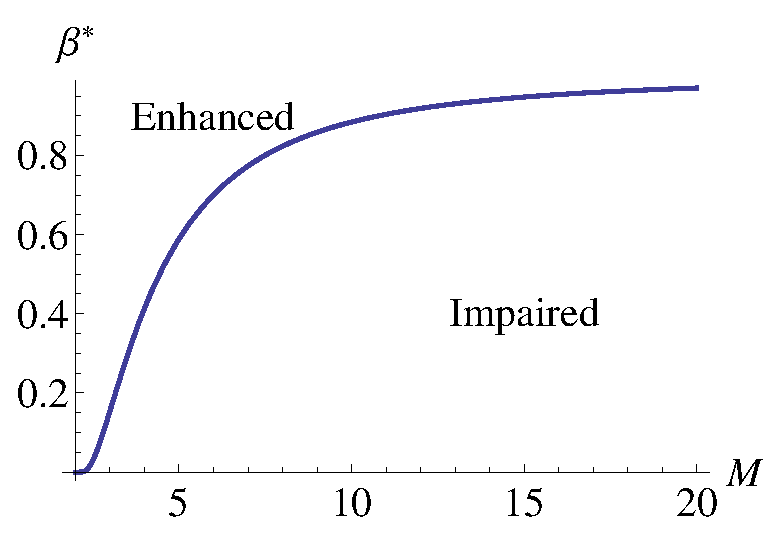
\includegraphics[width=7cm]{multistate_betastar.eps}}\label{fig:multistate_betastar}
  \item\aligntop{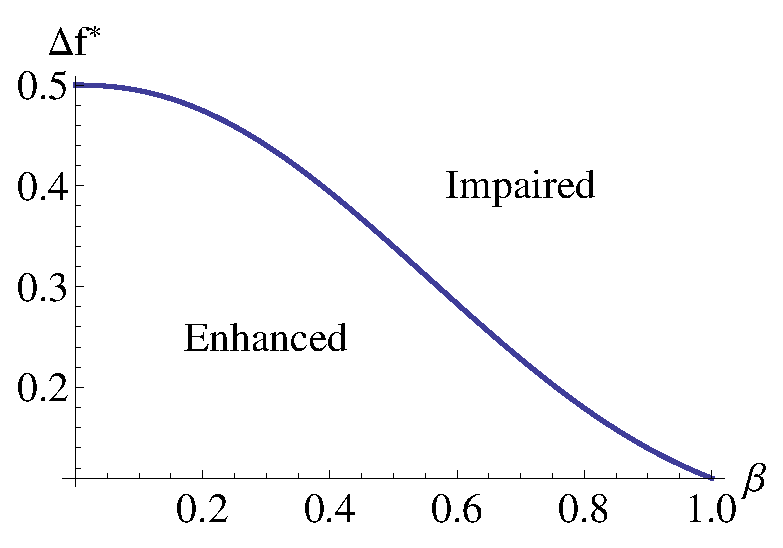
\includegraphics[width=7cm]{multistate_deltafstar.eps}}\label{fig:multistate_deltafstar}
 \end{myenuma}
 \end{center}
  \caption[The functions $\beta^*(M)$ and $\Delta f^*(\beta,M)$]{The functions (\ref{fig:multistate_betastar}) $\beta^*(M)$, which describes when the \KO\ models have impaired learning, and (\ref{fig:multistate_deltafstar}) $\Delta f^*(\beta,M)$ for $M=10$, which describes when pre-training enhances learning.}\label{fig:multistate_star}
\end{figure}

In conclusion, if we choose $\beta<\beta^*(M)$, $\Delta f > \Delta f^*(1,M)$ and look at intermediate time-scales, we will see that the \KO\ models learn slower than wild-type without pre-training, and that pre-training speeds up learning in the \KO\ models but slows it down in the wild-type.
However, in this case pre-training proceeds much faster in the \KO\ models than wild-type (see \autoref{fig:multistate_med}\ref{fig:multistate_med_learn} and \autoref{fig:multistate_strong}\ref{fig:multistate_strong_learn}, lower curves), which is \emph{not} seen in the experiment.

Now consider what would happen if we did not treat gain-increase and gain-decrease symmetrically.
Let us set $f\pot\dec = f\pot\norm - \overline{\Delta f}$.
Then, \eqref{eq:multiKOpre} becomes
%
\begin{equation}\label{eq:multiKOdiffpre}
\begin{aligned}
  \Phi &= 2\prn{\Delta f + \overline{\Delta f}} q \, \frac{(1-2\overline{\Delta f}) - \beta(1+2\overline{\Delta f})}
          {(1-2\overline{\Delta f})^M - \beta^M(1+2\overline{\Delta f})^M}   \,
          \brk{\beta (1-2\overline{\Delta f}) (1+2\overline{\Delta f})}^{M/2-1} \\
       &= 2\prn{\Delta f + \overline{\Delta f}} q\,\frac{(1-\beta)\beta^{M/2-1}}{1-\beta^M} + \CO(\Delta f,\overline{\Delta f})^2.
\end{aligned}
\end{equation}
%
We can then look at the wild-type by setting $\beta=1$:
%
\begin{equation}\label{eq:multiWTdiffpre}
\begin{aligned}
  \Phi &= 8\,\overline{\Delta f}\prn{\Delta f + \overline{\Delta f}} q \,
          \frac{(1-2\overline{\Delta f})^{M/2-1} (1+2\overline{\Delta f})^{M/2-1} }
          {{(1+2\overline{\Delta f})^M - (1-2\overline{\Delta f})^M}}   \\
       &= \frac{2\prn{\Delta f + \overline{\Delta f}} q}{M} + \CO(\Delta f,\overline{\Delta f})^2.
\end{aligned}
\end{equation}
%

We can see from these formulae that, if we want pre-training to impair learning in wild-type, but enhance it in the \KO\ models, the important thing is to have \emph{strong pre-training}, not strong training.
Thus, removing the symmetry between gain-increase and gain-decrease will not help with the most unrealistic feature of this model -- the fact that pre-training proceeds much faster in the \KO\ models than wild-type.

Finally, we note that, in the case of medium or strong pre-training, we see positive curvature in the learning curve after pre-training for a longer time in wild-type than in the \KO\ models (see \autoref{fig:multistate_med}\ref{fig:multistate_med_learnS} and \autoref{fig:multistate_strong}\ref{fig:multistate_strong_learnS}, dashed curves).
This is due to the mass of probability at the right end of the chain (see \autoref{fig:multistate_med}\ref{fig:multistate_med_eq} and \autoref{fig:multistate_strong}\ref{fig:multistate_strong_eq}, red trace) that is unable to contribute to change in synaptic weight until it has drifted to the centre.
This will last for a shorter time in the \KO\ models, due to the enhanced transitions.
This will not be a feature of any of the other models that we study here.
Now, the curvature can be changed by the nonlinear relation between synaptic weight and VOR gain, but both curves would be affected in the same way.
The difference in these two curvatures is therefore a good feature of this model.


\subsection{Two-state model}\label{sec:binary}


\resultsfign{two-state model}{binary}


The results of simulations of the two-state model can be seen in \autoref{fig:binary}.
However, this model can be solved exactly:
%
\begin{multline}\label{eq:binarysol}
  \eq = \frac{(f\dep q\dep, f\pot q\pot)}{\lambda},
  \qquad
  \pr(t) = \eq + (\pr(t)-\eq)\e^{-\lambda rt},\\
  \qquad \text{where} \quad
  \lambda = f\pot q\pot + f\dep q\dep.
\end{multline}
%
But it is easier to just substitute $M=2$ into the formulae in \autoref{sec:multistate}.
In this case, the initial rate of change and the total change encapsulate the whole solution, as there is only a single exponential decay.

First, consider the wild-type, for which $q\pot=q\dep=q$.
Without pre-training:
%
\begin{equation}\label{eq:binWTnopre}
  \Phi = {\Delta f}\, q.
\end{equation}
%
With pre-training:
%
\begin{equation}\label{eq:binWTpre}
\begin{aligned}
  \Phi &= 2{\Delta f}\, q.
\end{aligned}
\end{equation}
%
So, we see that pre-training will always speed up learning, unlike what is seen in the experiment.
This can be seen in \autoref{fig:binary}\ref{fig:binary_learnS} (black curves).

Now, consider the \KO\ models, for which we define $\beta=q\pot/q\dep<1$, and we set $q\pot=q$.
Without pre-training:
%
\begin{equation}\label{eq:binKOnopre}
  \Phi = \frac{2{\Delta f}\, q}{1+\beta},
\end{equation}
%
which is always larger that \eqref{eq:binWTnopre}, unlike what is seen in the experiment.
This is also seen in \autoref{fig:binary}\ref{fig:binary_learn},\ref{fig:binary_learnS} (solid curves).
As discussed above (below \eqref{eq:multiKOnopre}), the larger value of $q\dep=q/\beta$ has two effects.
Smaller $\beta$ will increase the probability of depression, speeding up learning, but it will also decrease the probability of being ready for depression, slowing down learning.
For the serial model, we argued that the first effect goes like $1/\beta$, whereas the second goes like $\beta^{M/2}$ to leading order.
Here $M=2$, so the leading part of the two effects will cancel.
The subleading effects (the normalisation of the probabilities) are responsible for the faster learning in the \KO\ models.

With pre-training:
%
\begin{equation}\label{eq:binKOpre}
\begin{aligned}
  \Phi &= 4{\Delta f}\, q \, \frac{(1-2\Delta f) - \beta(1+2\Delta f)}
          {(1-2\Delta f)^2 - \beta^2(1+2\Delta f)^2}.
\end{aligned}
\end{equation}
%
As we've already ruled out this model, we won't waste any time analysing this formula.

We made a number of assumptions in our analysis so far.
Before we declare this model to be falsified, we should think about what would happen if we relaxed these assumptions and explored a larger parameter space.

First, we assumed that the wild type had symmetric potentiation and depression.
Relaxing this assumption would correspond modelling the wild-type like the \KO\ mice, but with a different value for $\beta$.
We will still have $\beta\ko<\beta\wt$, and looking at \eqref{eq:binKOnopre} tell us that we would still have faster learning in the \KO\ models.

Secondly, we assumed that there would be equal rates of potentiation and depression in the untrained situation.
However, relaxing this assumption merely changes \eqref{eq:binKOnopre} to
%
\begin{equation}\label{eq:binKOnoprediff}
  \Phi = \frac{{\Delta f}\, q}{f\dep+\beta f\pot} = \frac{{\Delta f}\, q\pot q\dep}{f\dep q\dep+ f\pot q\pot}.
\end{equation}
%
This will not change our conclusions either.

As we didn't need the pre-training paradigm to rule out this model, we don't need to look at removing the symmetry between gain-increase and decrease.

The only thing we have to worry about is when the wild-type catches up with the \KO\ models.
As the total change will be larger for the wild-type than \KO\ models, it must overtake eventually.
If this happens early enough, the initial period, where the \KO\ models learns faster than wild-type, would not be seen in the experiment.
However, the timescale for this crossover would be similar to the timescale of the exponentials.
In the data, it looks like that timescale is longer than the gaps between successive measurements, so we needn't worry about this.

Intuitively, this model is missing two features of the \hyperref[sec:multistate]{serial model}.
First, it does not have the exponential amplification of the effect of initial saturation bias because this model does not have a chain of states for the distribution to decay across.
Second, it does not have the metaplastic effect where repeated potentiation makes future depression harder, as potentiation will merely increase the number of potentiated synapses.


\subsection{Multistate model}\label{sec:multistate_lin}

\resultsfign{multistate model}{multistate_lin}


In this section, we will consider the multistate model as originally defined in \cite{amit1994learning}, \ie with linearly varying synaptic weight:
%
\begin{equation}\label{eq:multistateLinWeight}
  \w_i = \frac{2i-M-1}{M-1}.
\end{equation}
%
The numerical results can be seen in \autoref{fig:multistate_lin}, but we can get some analytic insight into this model as well.
In essence, this model is like a series of two-state models attached to each other, in contrast to the serial model for which the synaptic weight only changes between one of the pairs of states.


The equilibrium distribution, \eqref{eq:mutltieq}, still applies.
However, now the rate of change of our learning metric, \eqref{eq:learning}, will be proportional to the sum of the net fluxes between adjacent states:
%
\begin{equation}\label{eq:multiLinFlux}
  \begin{aligned}
    \Phi &= \sum_{i=1}^{M-1} \eq_{i+1} f'{}\dep q\dep - \eq_i f'{}\pot q\pot
         &= \sum_{i=1}^{M-1} \eq_i (\alpha-\alpha') f'{}\dep q\dep \\
         &= \frac{1-\alpha^{M-1}}{1-\alpha^M} \, (\alpha-\alpha') f'{}\dep q\dep.
  \end{aligned}
\end{equation}
%

First, consider the wild-type, for which $q\pot=q\dep=q$.
Without pre-training:
%
\begin{equation}\label{eq:multiLinWTnopre}
  \Phi = 2{\Delta f}\,q\,\frac{M-1}{M},
\end{equation}
%
where, once more, we should note that $\Delta f<0$.
With pre-training:
%
\begin{equation}\label{eq:multiLinWTpre}
\begin{aligned}
  \Phi &= 4{\Delta f}\, q \, \frac{(1+2\Delta f)^{M-1} - (1-2\Delta f)^{M-1}}
          {(1+2\Delta f)^M - (1-2\Delta f)^M} \\
       &= {4{\Delta f}\, q}\,\frac{M-1}{M} + \CO(\Delta f)^2.
\end{aligned}
\end{equation}
%

Now, consider the \KO\ models, for which we define $\beta=q\pot/q\dep<1$, and we set $q\pot=q$.
Without pre-training:
%
\begin{equation}\label{eq:multiLinKOnopre}
  \Phi = 2{\Delta f}\, q\,\frac{1-\beta^{M-1}}{1-\beta^M}.
\end{equation}
%
This decreases monotonically in the interval $\beta\in[0,1]$, therefore this will always be greater than \eqref{eq:multiLinWTnopre}.
This means that the \KO\ models will initially learn faster than the wild-type.
However, as the wild-type will eventually catch up, and this can happen very quickly, as seen in \autoref{fig:multistate_lin}\ref{fig:multistate_lin_learn},\ref{fig:multistate_lin_learnS} (solid curves).

With pre-training:
%
\begin{equation}\label{eq:multiLinKOpre}
\begin{aligned}
  \Phi &= 4{\Delta f}\, q \, \frac{(1-2\Delta f)^{M-1} - \beta^{M-1}(1+2\Delta f)^{M-1}}
          {(1-2\Delta f)^M - \beta^M(1+2\Delta f)^M} \\
       &= 4{\Delta f}\, q\,\frac{1-\beta^{M-1}}{1-\beta^M} + \CO(\Delta f)^2.
\end{aligned}
\end{equation}
%
The ratio of this to \eqref{eq:multiLinKOnopre} takes its minimum value at the upper end of the interval $\Delta f \in \brk{0,\half}$, where it takes the value
%
\begin{equation}\label{eq:multiLinprenopre}
  \frac{\Phi_{\text{w/ pre}}}{\Phi_{\text{w/o pre}}} = \frac{1-\beta^M}{\beta-\beta^M}
   \longrightarrow \frac{M}{M-1} \quad \text{as} \quad \beta\to1,
\end{equation}
%
which is always greater than 1.
Therefore, pre-training will always enhance learning, for both \KO\ models and wild-type, as seen in \autoref{fig:multistate_lin}\ref{fig:multistate_lin_learnS}.


Like the \hyperref[sec:binary]{two state model}, this model is missing two features of the \hyperref[sec:multistate]{serial model}.
First, it does not have the amplification of the effect of initial saturation bias as every transition contributes to the learning signal, so the exponentially decaying distribution has no effect.
Second, it does not have the metaplastic effect where repeated potentiation makes future depression harder, as potentiation will merely increase the number of potentiated synapses without pushing them away from any boundary between strong and weak states.



\subsection{Pooled resource model}\label{sec:pooled}
%
%
%\resultsfig{pooled resource}{light depletion}{($q\lmin/q\lmax=0.75$)}{pooled_plenty}
%
%\resultsfig{pooled resource}{heavy depletion}{($q\lmin/q\lmax=0.125$)}{pooled_scarce}

\resultsfign{pooled resource}{pooled_deponly}


The results of simulations of the pooled resource model can be seen in \autoref{fig:pooled_deponly}.
It is difficult to study this model analytically.
However, the numerical results can helps us understand it qualitatively.

If we compare gain-increase learning in the \KO\ models to wild-type, there are two effects: the increased transition rates speed up learning, but the equilibrium distribution is shifted to the depressed side (compare \autoref{fig:pooled_deponly}\ref{fig:pooled_deponly_eq}: \ref{fig:pooled_deponly_eq_WT} and \ref{fig:pooled_deponly_eq_KO}, blue traces), where there are fewer synapses available for depression and resources are depleted.
When resource depletion is sufficiently severe, the second effect dominates and the \KO\ models learn slower than wild-type (see \autoref{fig:pooled_deponly}\ref{fig:pooled_deponly_learn},\ref{fig:pooled_deponly_learnS}, solid curves), which matches what is seen in the experiment.

Gain-decrease pre-training lessens the second effect, and results in the \KO\ models learning faster than wild-type (see \autoref{fig:pooled_deponly}\ref{fig:pooled_deponly_learn},\ref{fig:pooled_deponly_learnS}), as seen in the experiment.

Gain-decrease pre-training will shift the distribution to the potentiated side, where there are more synapses available for depression and resources are more plentiful, for both the \KO\ models and wild type (see \autoref{fig:pooled_deponly}\ref{fig:pooled_deponly_eq}, red traces).
This means that the pre-trained animals will learn faster then the untrained one for both \KO\ models and wild-type (see \autoref{fig:pooled_deponly}\ref{fig:pooled_deponly_learnS}).
This differs from what is seen experimentally, where the pre-trained wild-type learns slower than the untrained one.

This model shares one feature of the \hyperref[sec:multistate]{serial model}.
The effect of initial saturation bias is amplified by resource depletion, allowing for impaired learning with enhanced plasticity.
However, it does not have the metaplastic effect where repeated potentiation makes future depression harder, in fact it shows the opposite effect due to resource replenishment, so it can never show impaired learning after pre-training.



\subsection{Cascade model}\label{sec:cascade}

\resultsfig{cascade}{short pre-training}{($rt_\text{pre}=20$)}{cascade_short}

\resultsfig{cascade}{long pre-training}{($rt_\text{pre}=100$)}{cascade_long}



The results of simulations of the cascade model can be seen in \autoref{fig:cascade_short} and \autoref{fig:cascade_long}.
It is difficult to study this model analytically.
However, the numerical results can helps us understand it qualitatively.

In both of these, we see that the \KO\ models are slower than wild-type without pre-training but faster with it.
This seems to be due to the fact that, without pre-training, very few synapses will be available for depression as most of them are already depressed (\autoref{fig:cascade_short}\ref{fig:cascade_short_eq}\ref{fig:cascade_short_eq_KO} and \ref{fig:cascade_short_pr}\ref{fig:cascade_short_pr_KO_nopre}).
With pre-training, some of them will now be potentiated (\autoref{fig:cascade_short}\ref{fig:cascade_short_eq}\ref{fig:cascade_short_eq_KO} and \ref{fig:cascade_short_pr}\ref{fig:cascade_short_pr_KO_pre}), and the enhanced depression can speed up learning.

With shorter pre-training, we see that it speeds up learning in both wild-type and \KO\ models (see \autoref{fig:cascade_short}\ref{fig:cascade_short_learnS}), whereas experimentally this only happens for the \KO\ models.
This is due to the fact that pre-training results in more synapses being potentiated, and thus ready for depression, but does not push them far enough down the cascade for the lower transition probabilities to slow down learning (see \autoref{fig:cascade_short}\ref{fig:cascade_short_pr}\ref{fig:cascade_short_pr_WT_pre}).

We can see from \autoref{fig:cascade_long}\ref{fig:cascade_long_pr}\ref{fig:cascade_long_pr_WT_pre} that longer pre-training pushes the synapses further down the cascade, slowing down learning for the wild-type.
This effect is weaker for the \KO\ models, as the equilibrium distribution is not as heavily concentrated at the end (see \autoref{fig:cascade_long}\ref{fig:cascade_long_eq}\ref{fig:cascade_long_eq_KO}).


This model shares both features of the \hyperref[sec:multistate]{serial model}.
First, the effect of initial saturation bias is amplified by the exponential decay of transition probabilities away from the middle.
Second, it has the metaplastic effect where repeated potentiation makes future depression harder, also due to he exponential decay of transition probabilities.


\subsection{Non-uniform multistate model}\label{sec:nonuni}

\resultsfign{non-uniform multistate}{nonuni}



The results of simulations of the non-uniform multistate model can be seen in \autoref{fig:nonuni}.
It is difficult to study this model analytically.
However, the numerical results can helps us understand it qualitatively.

First, we see that the \KO\ models are slower than wild-type without pre-training, as seen experimentally.
This seems to be because the enhanced depression results in a greater fraction of synapses begin in states of weaker synaptic weight (see \autoref{fig:nonuni}\ref{fig:nonuni_eq}\ref{fig:nonuni_eq_KO}) where the depressing transitions have lower probability (see \autoref{fig:nonuni_model}).

However, gain-decrease pre-training will push synapses towards the states of stronger synaptic weight.
The wild-type will be pushed further that the \KO\ models, as the latter started further to the weaker side as explained above (compare \autoref{fig:nonuni}\ref{fig:nonuni_eq}\ref{fig:nonuni_eq_WT} and \ref{fig:nonuni_eq_KO}).
As the depressing transitions have lower probability for the strongest states (see \autoref{fig:nonuni_model}), this, in addition to the enhanced depression of the \KO\ models, will result in the \KO\ models learning faster than wild-type, as seen experimentally.

When comparing learning with and without gain-decrease pretraining, there are two effects to consider.
First, the pushing synapses towards the states of stronger synaptic weight, resulting in more synapses being available for depression, speeding up learning.
Second, it will also place synapses in states where transitions have lower probability, slowing down learning.
The second effect will be weaker in the \KO\ models than in wild-type, as they started further to the weaker side as explained above.
This means that, for appropriate parameter choices, gain-decrease pretraining can speed up learning in the \KO\ models, but also slow down learning in wild-type, as seen experimentally.

Like the \hyperref[sec:cascade]{cascade model}, this model also shares both features of the \hyperref[sec:multistate]{serial model}.
First, the effect of initial saturation bias is amplified by the exponential decay of transition probabilities away from the middle.
Second, it has the metaplastic effect where repeated potentiation makes future depression harder, also due to he exponential decay of transition probabilities.



\subsection{Parameter fitting}\label{sec:fit}

So far, we have only considered the comparisons listed at the start of \hyperref[sec:results]{this section}, as they raised important conceptual questions.
We have not considered the other two comparisons, the lack of difference between wild-type without pre-training and \KO\ with pretraining and between wild-type with pre-training and \KO\ without pretraining (the ``diagonal'' comparisons in the language of the main text), as they depend more on the values used for the parameters than on any conceptual issues.

However, for purely aesthetic purposes, we found parameter values performed reasonably in these other two comparisons two for the three models that could reproduce the correct qualitative results of the four important comparisons: the \hyperref[sec:multistate]{serial model}, the \hyperref[sec:cascade]{cascade model} and the \hyperref[sec:nonuni]{non-uniform multistate model}. The parameters are listed in \autoref{tab:fit} and the learning curves are shown in \autoref{fig:fit}.


\begin{table}
 \begin{center}
  \begin{tabularn}{|l|c|c|c|c|c|c|c|c|c|}
    \cline{1-10}
    % after \\: \hline or \cline{col1-col2} \cline{col3-col4} ...
    Model & \# states & \multicolumn{3}{c|}{parameter} & \multicolumn{3}{c|}{$f\dep$} & \multicolumn{2}{c|}{$rt$} \\
    \cline{3-10}
    & & pot & WT dep & \KO\ dep & base & inc & dec & train & pre \\

    \cline{1-10}
    Serial   & 10 & $0.12$  & $0.14$  & $0.2$  & 0.5 & 0.11 & 0.89 & 5  & 100  &\label{tr:serial_fit} \\
    Cascade  & 14 & $0.386$  & $0.398$  & $0.466$  & 0.522 & 0.63 & 0.002 & 1.5  & 200  &\label{tr:cascade_fit} \\
    Non-uni. & 12 & $0.4$    & $0.4$    & $0.53$   & 0.5 & 0.7 & 0.1 & 5  & 500  &\label{tr:nonuni_fit} \\
    \cline{1-10}
  \end{tabularn}
 \end{center}
  \caption{Parameters used to reproduce detailed experimental results. For the sewrial model, the parameter listed is the transition probability between adjacent states. For the cascade and non-uniform multistate models, the parameter is the ratio of adjacent transition probabilities.} \label{tab:fit}
\end{table}

\begin{figure}
 \begin{center}
 \begin{myenuma}
  \item\aligntop{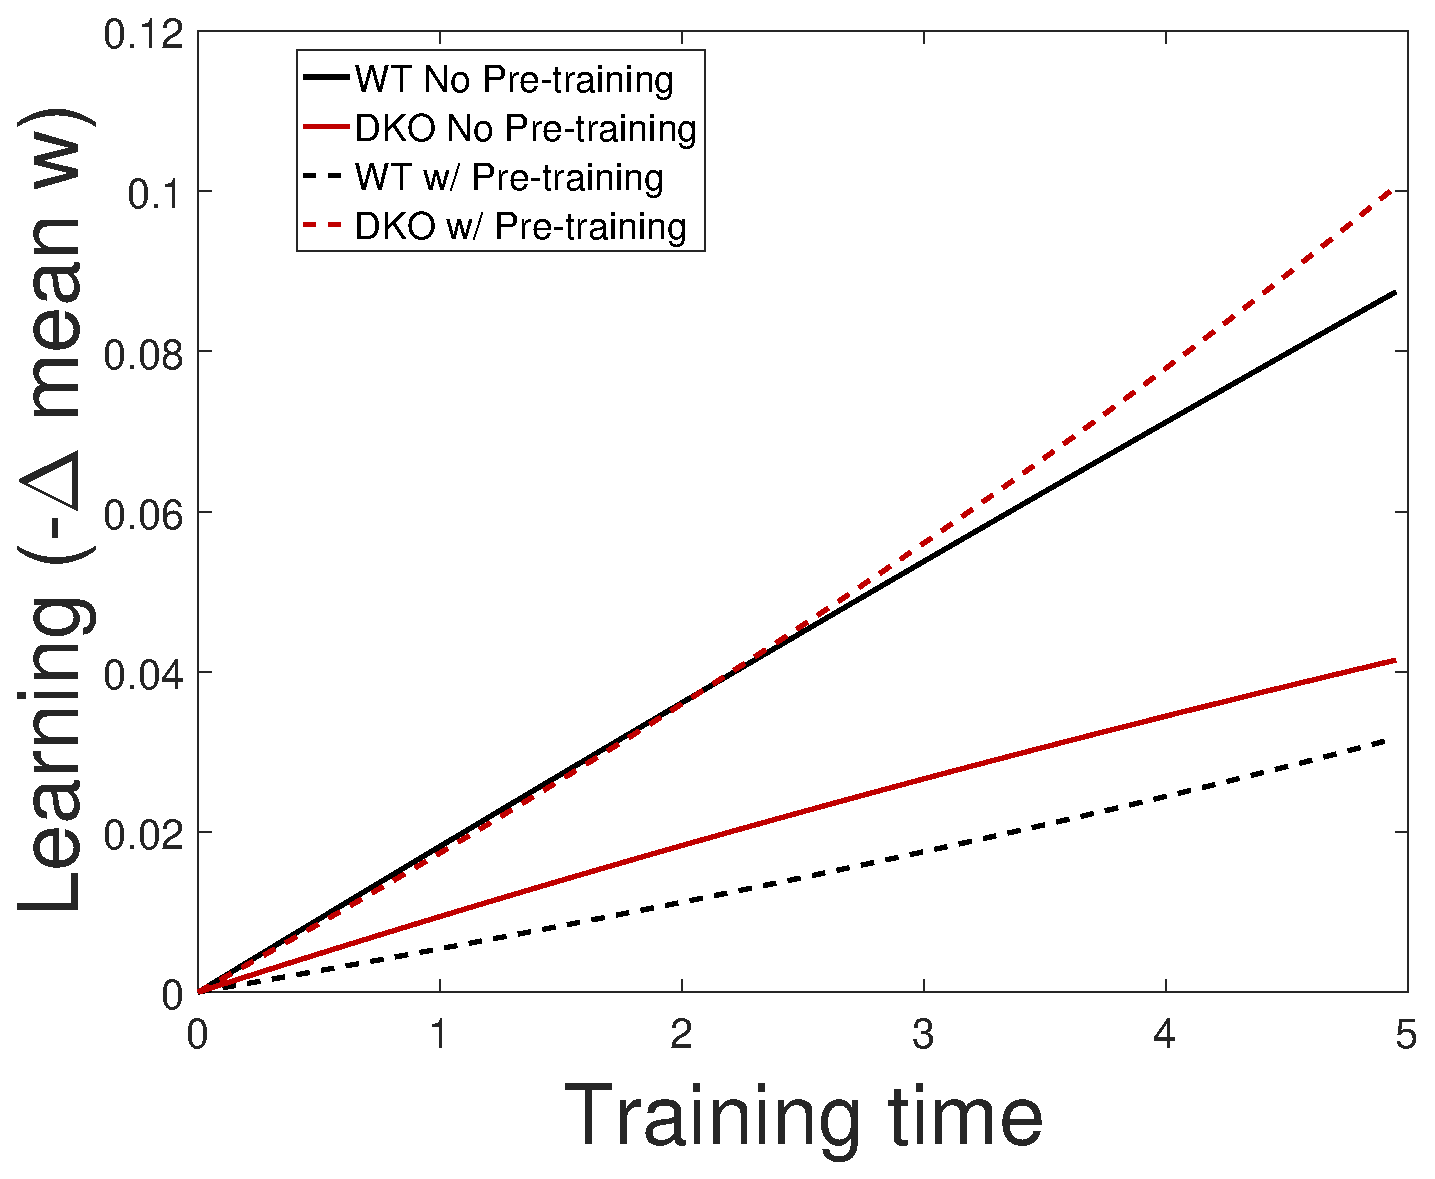
\includegraphics[width=4.5cm]{serial_fit_learnS.eps}}\label{fig:serial_fit}
  \item\aligntop{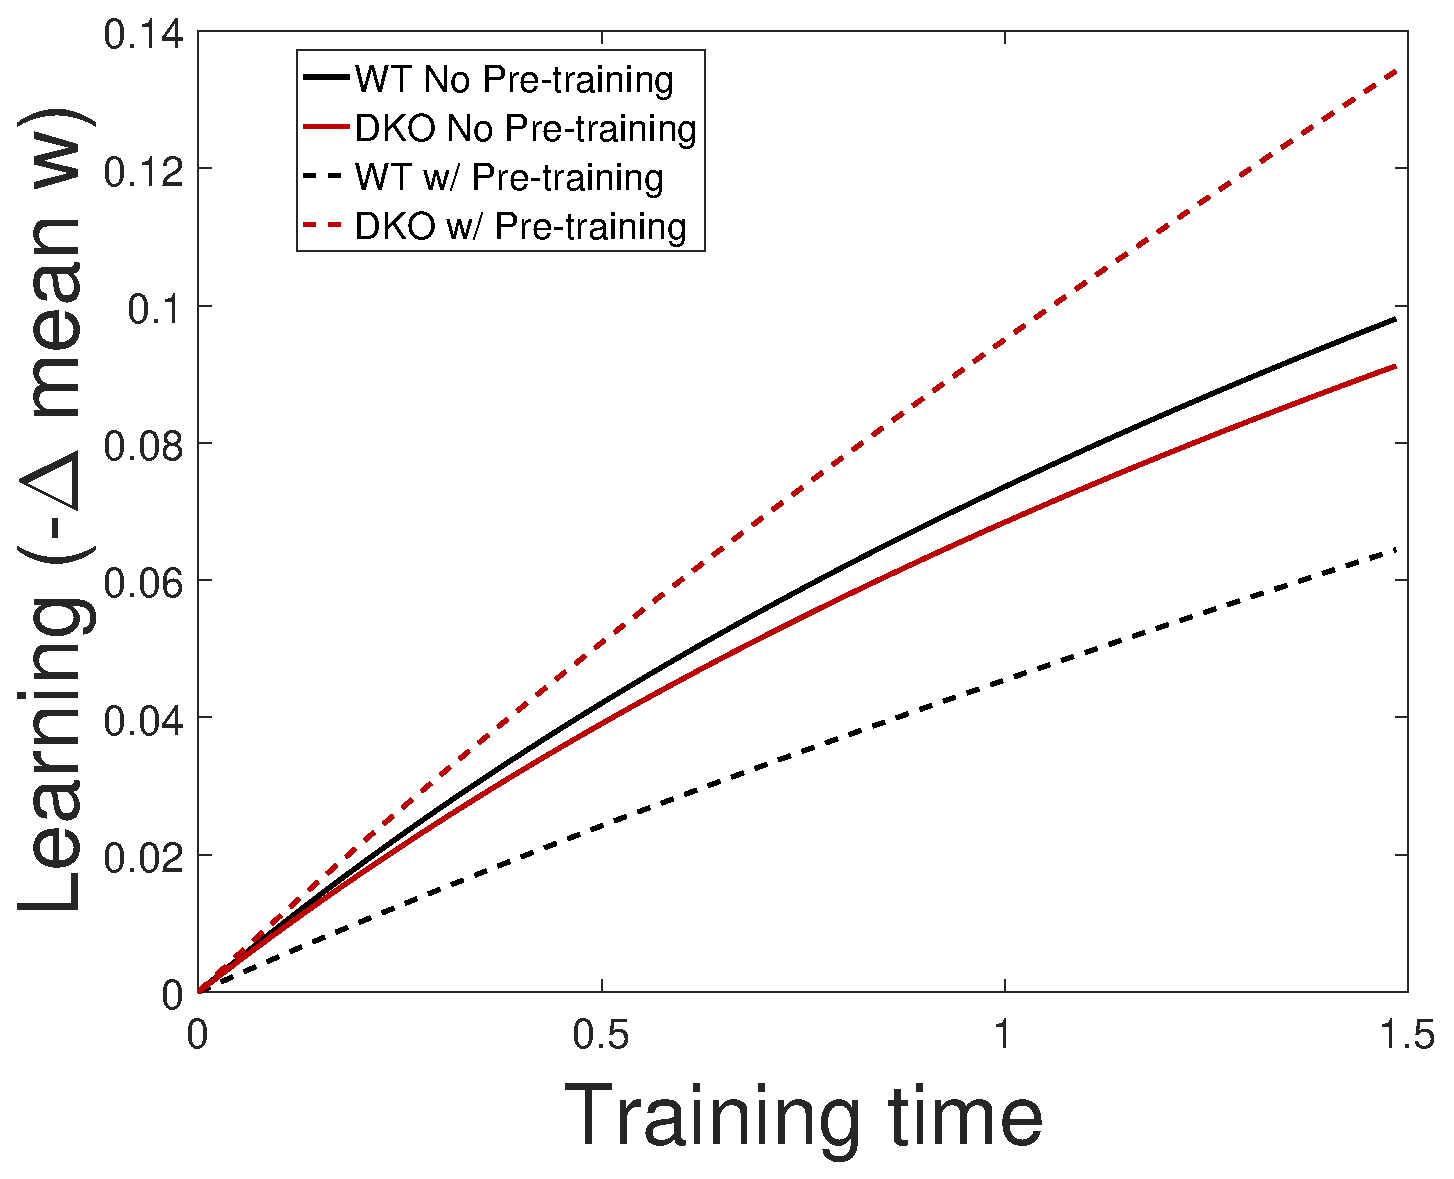
\includegraphics[width=4.5cm]{cascade_fit_learnS.eps}}\label{fig:cascade_fit}
  \item\aligntop{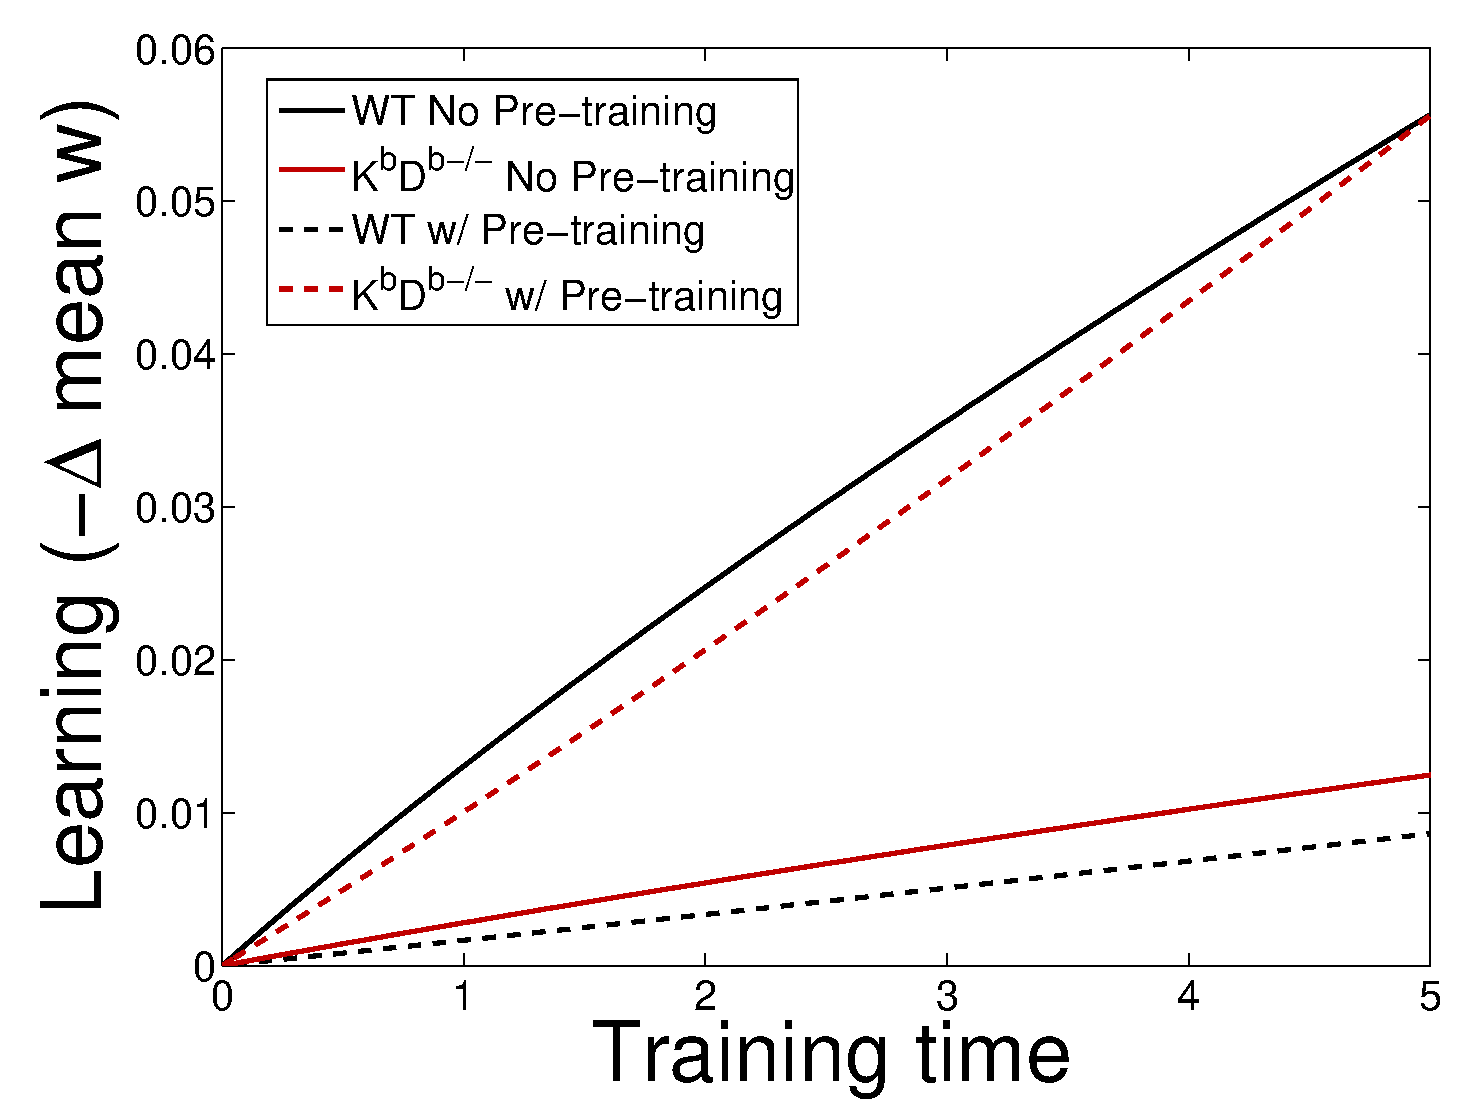
\includegraphics[width=4.5cm]{nonuni_fit_learnS.eps}}\label{fig:nonuni_fit}
 \end{myenuma}
 \end{center}
  \caption{Learning curves restricted to gain-increase training with parameters listed in \autoref{tab:fit}, for (\ref{fig:serial_fit}) the serial model, (\ref{fig:cascade_fit}) the cascade model, and (\ref{fig:nonuni_fit}) the non-uniform multistate model.}\label{fig:fit}
\end{figure}



%%%%%%%%%%%%%%%%%%%%%%%%%%%%%%%%%%%%%%%%%%%%%%%%%%%%%%%%%%%%%%%%%%%%%%%%%%

\bibliographystyle{utcaps_sl}
\bibliography{maths,neuro}

\end{document}
